\documentclass[10pt, compress]{beamer}

\usetheme{m}

\usepackage{booktabs}
\usepackage[scale=2]{ccicons}
\usepackage{minted}

\usemintedstyle{trac}

\usepackage{tikz}
\usepackage{tikz-qtree}
\usetikzlibrary{matrix,backgrounds, decorations.pathreplacing, automata, arrows}

\tikzset{onslide/.code args={<#1>#2}{%
  \only<#1>{\pgfkeysalso{#2}} % \pgfkeysalso doesn't change the path
}}
\tikzset{
  invisible/.style={opacity=0},
  visible on/.style={alt={#1{}{invisible}}},
  alt/.code args={<#1>#2#3}{%
    \alt<#1>{\pgfkeysalso{#2}}{\pgfkeysalso{#3}} % \pgfkeysalso doesn't change the path
  },
  blink/.style={onslide={<#1> mLightBrown}},
  appear/.style={visible on=<#1->, blink=#1}
}

\newcommand{\tdots}{\,.\,.\,} % in place of \ldots
\newcommand{\E}{\Sigma}
\newcommand{\Oh}{\mathcal{O}}
\newcommand{\cS}{\mathcal{S}}


\title{Algoritmos em Sequências}
\subtitle{Yan Soares Couto}
\date{2016}
\author{Orientadora: Cristina Gomes Fernandes}
\institute{Instituto de Matemática e Estatística}


\begin{document}

\maketitle

\begin{frame}[fragile]
  \frametitle{definição}

String~$S[1\tdots|S|]$: vetor em que cada elemento é de um alfabeto~$\E$ finito.

Em geral,~$\E = \{\text{a}, \text{b}, \ldots, \text{z}\}$.

\pause
\begin{center}
{\huge ``abracadabra''}
\end{center}

Substring de~$S$: subvetor de~$S$, por exemplo, {\large``cadab''}.

\end{frame}

\section{Palíndromos}

\begin{frame}[fragile]
  \frametitle{Palíndromos}
  
Palíndromo: string que coincide com seu reflexo (de trás pra frente)
  
\begin{center}
{\huge ``reviver''}
\end{center}

\alert{Problema:} Qual a maior substring de~$S$ que é um palíndromo?

\pause
\vspace{2ex}\textbf{Solução trivial:} Para cada posição~$i$ de~$S$, determinar o maior palíndromo par e ímpar com centro~$i$

Complexidade:~$\Oh(|S|^2)$.

\end{frame}

\begin{frame}[fragile]
\frametitle{Palíndromos ímpares}

Consideremos apenas palíndromos de tamanho ímpar.

Centro de palíndromo (ímpar): posição do meio

Ex: {\large ``reviver''} tem centro na letra~{\large i}.
\pause

Seja~$\alert{M[i]}$ é o maior inteiro tal que~$S[i-M[i]\tdots i+M[i]]$ é palíndromo.

\begin{center}
\hspace{-1ex}
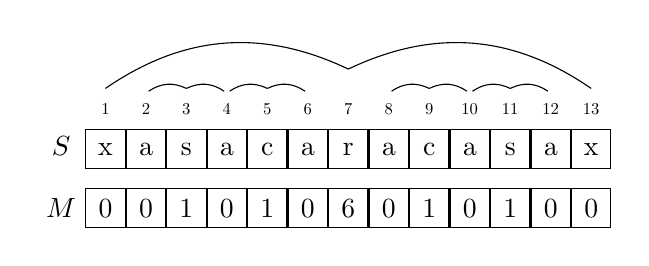
\begin{tikzpicture}
\matrix[matrix of nodes, nodes in empty cells,
row 1/.style={nodes={scale=.6, minimum size = 5mm}},
row 2/.style={nodes={draw, minimum size = 5mm}},
row 3/.style={nodes={minimum size = 2mm}},
row 4/.style={nodes={draw, minimum size = 5mm}},
row 2 column 1/.style={nodes={draw=none}},
row 4 column 1/.style={nodes={draw=none}}
] (array) {
    & 1 & 2 & 3 & 4 & 5 & 6 & 7 & 8 & 9 & 10 & 11 & 12 & 13 \\
$S$ & x & a & s & a & c & a & r & a & c & a & s & a & x \\
  &   &   &   &   &   &   &   &   &   &   &   &   &   \\
$M$ & 0 & 0 & 1 & 0 & 1 & 0 & 6 & 0 & 1 & 0 & 1 & 0 & 0 \\};

\path ([yshift=3]array-1-2.north) edge [bend left] ([yshift=10]array-1-8.north);
\path ([yshift=10]array-1-8.north) edge [bend left]  ([yshift=3]array-1-14.north);

\path ([yshift=2,xshift=1]array-1-3.north) edge [bend left] ([yshift=3]array-1-4.north);
\path ([yshift=3]array-1-4.north) edge [bend left] ([yshift=2,xshift=-1]array-1-5.north);

\path ([yshift=2,xshift=1]array-1-11.north) edge [bend left] ([yshift=3]array-1-12.north);
\path ([yshift=3]array-1-12.north) edge [bend left] ([yshift=2,xshift=-1]array-1-13.north);

\path ([yshift=2,xshift=1]array-1-5.north) edge [bend left] ([yshift=3]array-1-6.north);
\path ([yshift=3]array-1-6.north) edge [bend left] ([yshift=2,xshift=-1]array-1-7.north);

\path ([yshift=2,xshift=1]array-1-9.north) edge [bend left] ([yshift=3]array-1-10.north);
\path ([yshift=3]array-1-10.north) edge [bend left] ([yshift=2,xshift=-1]array-1-11.north);

\end{tikzpicture}

\pause
\alert{Como calcular M de forma rápida?}

\end{center}

\end{frame}

\begin{frame}[fragile]
\frametitle{Usando resultados anteriores}

Seja~$k$ tal que~$k < i$ e~$k + M[k] > i$.

Existe uma ``cópia'' da string em volta de~$i$ espelhada em~$k$, centrada na posição~$i' = 2k - i$.

\begin{center}
\begin{tikzpicture}
\matrix[matrix of nodes, nodes in empty cells,
row 1/.style={nodes={scale=.6, minimum size = 5mm}},
row 2/.style={nodes={draw, minimum size = 5mm}},
row 2 column 1/.style={nodes={draw=none}}
] (array) {
    & 1 & 2 & 3 & 4 & 5 & 6 & 7 & 8 & 9 & 10 & 11 & 12 & 13 \\
$S$ & x & a & s & a & c & a & r & a & c & a & s & a & x \\};

\path ([yshift=3]array-1-2.north) edge [bend left] ([yshift=10]array-1-8.north);
\path ([yshift=10]array-1-8.north) edge [bend left]  ([yshift=3]array-1-14.north);
\node at ([yshift=20]array-1-8.north) {$k$};
\path[dashed] ([yshift=15]array-1-8.north) edge (array-1-8.north);

\path ([yshift=-2]array-2-2.south) edge [bend right, draw=mLightBrown] ([yshift=-7]array-2-4.south);
\path ([yshift=-7]array-2-4.south) edge [bend right, draw=mLightBrown] ([yshift=-2]array-2-6.south);
\node at ([yshift=-15]array-2-4.south) {$i'$};
\path[dashed] ([yshift=-10]array-2-4.south) edge (array-2-4.south);


\path ([yshift=-2]array-2-10.south) edge [bend right, draw=mLightBrown] ([yshift=-7]array-2-12.south);
\path ([yshift=-7]array-2-12.south) edge [bend right, draw=mLightBrown] ([yshift=-2]array-2-14.south);
\node at ([yshift=-15]array-2-12.south) {$i$};
\path[dashed] ([yshift=-10]array-2-12.south) edge (array-2-12.south);
\end{tikzpicture}
\end{center}

A string destacada centrada em~$i'$ é o reflexo da string destacada centrada em~$i$.

\end{frame}

\begin{frame}[fragile]
\frametitle{Usando resultados anteriores - Caso 1}

String espelhada:~$S[i-(k+M[k]-i)\tdots i+(k+M[k]-i)]$.

Se essa string não é palíndromo ($M[i'] < k + M[k] - i$), então~${M[i] = M[i']}$.
%explicar ao apresentar

\begin{center}
\begin{tikzpicture}
\matrix[matrix of nodes, nodes in empty cells,
row 1/.style={nodes={scale=.6, minimum size = 5mm}},
row 2/.style={nodes={draw, minimum size = 5mm}},
row 2 column 1/.style={nodes={draw=none}}
] (array) {
    & 1 & 2 & 3 & 4 & 5 & 6 & 7 & 8 & 9 & 10 & 11 & 12 & 13 \\
$S$ & x & a & s & a & c & a & r & a & c & a & s & a & x \\};

\path ([yshift=3]array-1-2.north) edge [bend left] ([yshift=10]array-1-8.north);
\path ([yshift=10]array-1-8.north) edge [bend left]  ([yshift=3]array-1-14.north);
\node at ([yshift=20]array-1-8.north) {$k$};
\path[dashed] ([yshift=15]array-1-8.north) edge (array-1-8.north);

\path ([yshift=-2]array-2-2.south) edge [bend right, draw=mLightBrown] ([yshift=-7]array-2-4.south);
\path ([yshift=-7]array-2-4.south) edge [bend right, draw=mLightBrown] ([yshift=-2]array-2-6.south);
\node at ([yshift=-15]array-2-4.south) {$i'$};
\path[dashed] ([yshift=-10]array-2-4.south) edge (array-2-4.south);


\path ([yshift=-2]array-2-10.south) edge [bend right, draw=mLightBrown] ([yshift=-7]array-2-12.south);
\path ([yshift=-7]array-2-12.south) edge [bend right, draw=mLightBrown] ([yshift=-2]array-2-14.south);
\node at ([yshift=-15]array-2-12.south) {$i$};
\path[dashed] ([yshift=-10]array-2-12.south) edge (array-2-12.south);
\end{tikzpicture}

Nesse caso~$M[i] = M[i'] = 1$.
\end{center}

\end{frame}

\begin{frame}[fragile]
\frametitle{Usando resultados anteriores - Caso 2}

Se essa string é palíndromo ($M[i'] \geq k + M[k] - i$), temos que~$M[i] \geq k + M[k] - i$.

%explicar ao apresentar

\begin{center}
\begin{tikzpicture}
\matrix[matrix of nodes, nodes in empty cells,
row 1/.style={nodes={scale=.6, minimum size = 5mm}},
row 2/.style={nodes={draw, minimum size = 5mm,anchor=center}},
row 2 column 1/.style={nodes={draw=none}}
] (array) {
    & 1 & 2 & 3 & 4 & 5 & 6 & 7 & 8 & 9 & 10 & 11 & 12 & 13 & 14 & 15 \\
$S$ & k & c & a & s & a & c & a & r & a & c & a & s & a & c & z \\};

\path ([yshift=3]array-1-3.north) edge [bend left] ([yshift=10]array-1-9.north);
\path ([yshift=10]array-1-9.north) edge [bend left]  ([yshift=3]array-1-15.north);
\node at ([yshift=20]array-1-9.north) {$k$};
\path[dashed] ([yshift=15]array-1-9.north) edge (array-1-9.north);

\path ([yshift=-2]array-2-3.south) edge [bend right, draw=mLightBrown] ([yshift=-7]array-2-5.south);
\path ([yshift=-7]array-2-5.south) edge [bend right, draw=mLightBrown] ([yshift=-2]array-2-7.south);
\node at ([yshift=-15]array-2-5.south) {$i'$};
\path[dashed] ([yshift=-10]array-2-5.south) edge (array-2-5.south);


\path ([yshift=-2]array-2-11.south) edge [bend right, draw=mLightBrown] ([yshift=-7]array-2-13.south);
\path ([yshift=-7]array-2-13.south) edge [bend right, draw=mLightBrown] ([yshift=-2]array-2-15.south);
\node at ([yshift=-15]array-2-13.south) {$i$};
\path[dashed] ([yshift=-10]array-2-13.south) edge (array-2-13.south);
\end{tikzpicture}

Nesse caso~$M[i] = 2$ e $M[i'] = 2$.
\end{center}

Pode ocorrer de $$M[i] = k + M[k] - i = M[i']$$ { ou...}

\end{frame}

\begin{frame}[fragile]
\frametitle{Usando resultados anteriores - Caso 2}
\addtocounter{framenumber}{-1}

Se essa string é palíndromo ($M[i'] \geq k + M[k] - i$), temos que~$M[i] \geq k + M[k] - i$.
%explicar ao apresentar

\begin{center}
\begin{tikzpicture}
\matrix[matrix of nodes, nodes in empty cells,
row 1/.style={nodes={scale=.6, minimum size = 5mm}},
row 2/.style={nodes={draw, minimum size = 5mm,anchor=center}},
row 2 column 1/.style={nodes={draw=none}}
] (array) {
    & 1 & 2 & 3 & 4 & 5 & 6 & 7 & 8 & 9 & 10 & 11 & 12 & 13 & 14 & 15 \\
$S$ & k & c & a & s & a & c & a & r & a & c & a & s & a & c & a \\};

\path ([yshift=3]array-1-3.north) edge [bend left] ([yshift=10]array-1-9.north);
\path ([yshift=10]array-1-9.north) edge [bend left]  ([yshift=3]array-1-15.north);
\node at ([yshift=20]array-1-9.north) {$k$};
\path[dashed] ([yshift=15]array-1-9.north) edge (array-1-9.north);

\path ([yshift=-2]array-2-3.south) edge [bend right, draw=mLightBrown] ([yshift=-7]array-2-5.south);
\path ([yshift=-7]array-2-5.south) edge [bend right, draw=mLightBrown] ([yshift=-2]array-2-7.south);
\node at ([yshift=-15]array-2-5.south) {$i'$};
\path[dashed] ([yshift=-10]array-2-5.south) edge (array-2-5.south);


\path ([yshift=-2]array-2-11.south) edge [bend right, draw=mLightBrown] ([yshift=-7]array-2-13.south);
\path ([yshift=-7]array-2-13.south) edge [bend right, draw=mLightBrown] ([yshift=-2]array-2-15.south);
\node at ([yshift=-15]array-2-13.south) {$i$};
\path[dashed] ([yshift=-10]array-2-13.south) edge (array-2-13.south);
\end{tikzpicture}

Nesse caso~$M[i] = 3$ e $M[i'] = 2$.
\end{center}

{ ou...} $$M[i] > k + M[k] - i = M[i']$$


\end{frame}

\begin{frame}[fragile]
\frametitle{Usando resultados anteriores - Caso 2}
\addtocounter{framenumber}{-1}

Se essa string é palíndromo ($M[i'] \geq k + M[k] - i$), temos que~$M[i] \geq k + M[k] - i$.
%explicar ao apresentar

\begin{center}
\begin{tikzpicture}
\matrix[matrix of nodes, nodes in empty cells,
row 1/.style={nodes={scale=.6, minimum size = 5mm}},
row 2/.style={nodes={draw, minimum size = 5mm,anchor=center}},
row 2 column 1/.style={nodes={draw=none}}
] (array) {
    & 1 & 2 & 3 & 4 & 5 & 6 & 7 & 8 & 9 & 10 & 11 & 12 & 13 & 14 & 15 \\
$S$ & a & c & a & s & a & c & a & r & a & c & a & s & a & c & k \\};

\path ([yshift=3]array-1-3.north) edge [bend left] ([yshift=10]array-1-9.north);
\path ([yshift=10]array-1-9.north) edge [bend left]  ([yshift=3]array-1-15.north);
\node at ([yshift=20]array-1-9.north) {$k$};
\path[dashed] ([yshift=15]array-1-9.north) edge (array-1-9.north);

\path ([yshift=-2]array-2-3.south) edge [bend right, draw=mLightBrown] ([yshift=-7]array-2-5.south);
\path ([yshift=-7]array-2-5.south) edge [bend right, draw=mLightBrown] ([yshift=-2]array-2-7.south);
\node at ([yshift=-15]array-2-5.south) {$i'$};
\path[dashed] ([yshift=-10]array-2-5.south) edge (array-2-5.south);


\path ([yshift=-2]array-2-11.south) edge [bend right, draw=mLightBrown] ([yshift=-7]array-2-13.south);
\path ([yshift=-7]array-2-13.south) edge [bend right, draw=mLightBrown] ([yshift=-2]array-2-15.south);
\node at ([yshift=-15]array-2-13.south) {$i$};
\path[dashed] ([yshift=-10]array-2-13.south) edge (array-2-13.south);
\end{tikzpicture}

Nesse caso~$M[i] = 2$ e $M[i'] = 3$.
\end{center}

{ ou...} $$M[i] = k + M[k] - i < M[i']$$


\end{frame}


\begin{frame}[fragile]
\frametitle{Algoritmo}

Ideia: Usar os valores~$M[i']$ para~$i' < i$ para facilitar o cálculo de~$M[i]$.

Usar o~$k$ que maximiza~${k + M[k]}$ para partir da melhor cota inferior para~$M[i]$.

É possível manter o~$k$ ótimo enquanto calculamos os valores de~$M$, e obter uma implementação que consome tempo~$\Oh(|S|)$.

\end{frame}

\begin{frame}[fragile]
\frametitle{Finalização, e palíndromos pares}

Podemos assim descobrir a maior substring que é um palíndromo de tamanho \textbf{ímpar}.

É possível adaptar o algoritmo para lidar com palíndromos pares.

Por exemplo, modifique a string~$S$ para~${\textsc{Fill}(S) = S[1]\$S[2]\$\ldots\$S[|S|]}$. Os palíndromos de~$S$ se transformam em palíndromos ímpares em~$\textsc{Fill}(S)$.

\begin{center}
{\huge abba $\rightarrow$ a\$b\$b\$a}
\end{center}

\end{frame}

\section{Tries}

\begin{frame}[fragile]
\frametitle{Definição}

\textbf{Trie}: árvore enraizada que armazena um conjunto de strings.

Strings são representadas como caminhos a partir da raiz.

\end{frame}

\begin{frame}[fragile]
\frametitle{Construção}

\begin{center}
\begin{tikzpicture}[sibling distance=25pt]
\Tree [.{}
\edge[appear=2]; [.\node[appear=2,blink=6]{m}; \edge[appear=3]; [.\node[appear=3,blink=7]{a}; \edge[appear=8]; [.\node[appear=8]{m}; \edge[appear=9]; [.\node[appear=9]{a}; \edge[appear=10]; [.\node[appear=10]{t}; \edge[appear=11]; \node[appear=11,draw]{a}; ] ] ] \edge[appear=4]; [.\node[appear=4]{t};  \edge[appear=5]; \node[appear=5, draw]{a}; ] ] ]
%
%
\edge[appear=12]; [.\node[appear=12,blink=16, blink=18]{o}; \edge[appear=13]; [.\node[appear=13,onslide={<17-> draw}, blink=17]{i}; \edge[appear=14]; [.\node[appear=14]{t}; \edge[appear=15]; \node[appear=15,draw]{o}; ] ] \edge[appear=19]; [.\node[appear=19]{m}; \edge[appear=20]; [.\node[appear=20]{a}; \edge[appear=21]; \node[appear=21,draw]{r}; ] ] ]
]
\end{tikzpicture}

Adicionando \only<1-5>{\large ``mata''.} \only<6-11>{\large ``mamata''.} \only<12-15>{\large ``oito''.} \only<16-17>{\large ``oi''.} \only<18-22>{\large ``omar''.}
\end{center}

\end{frame}

\begin{frame}[fragile]
\frametitle{Usos}

Construir uma trie para~$\cS = \{S_1, \ldots, S_k\}$ consome tempo~$\Oh(\sum\limits_{i=1}^k{|S_i|})$.

Com esta trie, podemos realizar:
\begin{description}
\item [\textsc{Contains}$(S)$] Determina se~$S \in \cS$.
\item [\textsc{LCP}$(S)$] Determina o maior prefixo comum de~$S$ com alguma string de~$\cS$.
\end{description}

Consumo de tempo:~$\Oh(|S|)$.


\end{frame}

\section{Aho-Corasick}

\begin{frame}[fragile]
\frametitle{Introdução}

\alert{Problema:} Determine todas as ocorrências de todas as strings de~$\cS = \{S_1, \ldots, S_k\}$ em~$T$.
\vspace{2ex}

\pause

Para cada sufixo~$T[i\tdots |T|]$, usando uma trie, determinamos as strings de~$\cS$ que ocorrem \textbf{no início} de~$T[i\tdots |T|]$.

Isso leva tempo~$\Oh(|T|^2 + \sum\limits_{i=1}^k{|S_i||\E|})$.

\end{frame}

\begin{frame}[fragile]
\frametitle{Links de falha}

No KMP: função prefixo guarda, para cada~$i$, o comprimento do maior prefixo de~$T$ que é sufixo próprio de~$T[1\tdots i]$.

\begin{center}
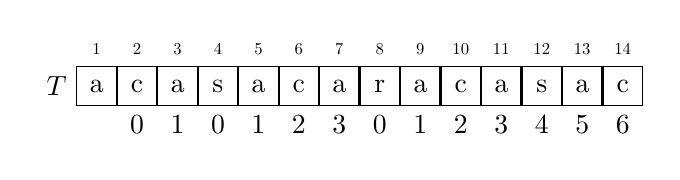
\begin{tikzpicture}
\matrix[matrix of nodes, nodes in empty cells,
row 1/.style={nodes={scale=.6, minimum size = 5mm}},
row 2/.style={nodes={draw, minimum size = 5mm,anchor=center}},
row 2 column 1/.style={nodes={draw=none}}
] (array) {
    & 1 & 2 & 3 & 4 & 5 & 6 & 7 & 8 & 9 & 10 & 11 & 12 & 13 & 14 \\
$T$ & a & c & a & s & a & c & a & r & a & c & a & s & a & c \\
    &   & 0 & 1 & 0 & 1 & 2 & 3 & 0 & 1 & 2 & 3 & 4 & 5 & 6 \\
};

\end{tikzpicture}
\end{center}

\pause
Em Tries: para cada nó~$v$, guarda o nó mais profundo cuja string seja um sufixo próprio da string de~$v$.

\begin{center}
\emph{\huge link de falha}
\end{center}

%Ou seja, queremos para cada prefixo~$S_1[1\tdots i]$ de \textbf{alguma} string de~$\cS$, queremos encontrar o maior prefixo~$S_2[1\tdots j]$ de \textbf{alguma} (possivelmente outra) string de~$\cS$ tal que~$S_2[1\tdots j]$ seja sufixo próprio de~$S_1[1\tdots i]$.

\end{frame}

\begin{frame}[fragile]
\frametitle{Links de falha}

Para cada nó~$v$, guardar o nó mais profundo cuja string seja um \alert{sufixo próprio} da string de~$v$.

\begin{center}
\centering
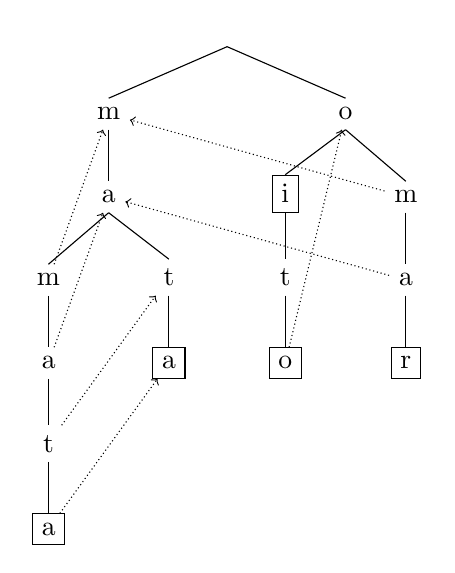
\begin{tikzpicture}[sibling distance=30pt]
\Tree [.{}
[.\node(m){m}; [.\node(ma){a}; [.\node(mam){m}; [.\node(mama){a}; [.\node(mamat){t}; \node[draw](mamata){a}; ] ] ] [.\node(mat){t}; \node[draw](mata){a}; ] ] ]
[.\node(o){o}; [.\node[draw](oi){i}; [.\node(oit){t}; \node[draw](oito){o}; ] ] [.\node(om){m}; [.\node(oma){a}; \node[draw](omar){r}; ] ] ]
]
%\draw[semithick,->] (t)..controls +(south west:5) and +(south:5)..(wh);
\draw[densely dotted,->] (mamata) -- (mata);
\draw[densely dotted,->] (mamat) -- (mat);
\draw[densely dotted,->] (mama) -- (ma);
\draw[densely dotted,->] (mam) -- (m);
\draw[densely dotted,->] (oito) -- (o);
\draw[densely dotted,->] (oma) -- (ma);
\draw[densely dotted,->] (om) -- (m);
\end{tikzpicture}
\end{center}

\end{frame}

\begin{frame}[fragile]
\frametitle{Algoritmo}

Para cada prefixo~$T[1\tdots i]$, determinar o maior prefixo~$S[1\tdots j]$ de alguma string de~$\cS$ que é sufixo de~$T[1\tdots i]$.

\end{frame}

\begin{frame}[fragile]
\frametitle{Algoritmo}

\begin{center}

\begin{tikzpicture}
\matrix[matrix of nodes, nodes in empty cells,
row 1/.style={nodes={scale=.6, minimum size = 5mm}},
row 2/.style={nodes={draw, minimum size = 5mm,anchor=center}},
row 2 column 1/.style={nodes={draw=none}}
] (array) {
    & \node[onslide={<2> mLightBrown}]{1}; & \node[onslide={<3> mLightBrown}]{2}; & \node[onslide={<4> mLightBrown}]{3}; & \node[onslide={<5> mLightBrown}]{4}; & \node[onslide={<6> mLightBrown}]{5}; & \node[onslide={<7> mLightBrown}]{6}; & \node[onslide={<8> mLightBrown}]{7}; & \node[onslide={<9> mLightBrown}]{8}; \\
$T$ & o & m & a & m & a & t & a & m \\
};

\end{tikzpicture}


\begin{tikzpicture}[sibling distance=30pt]
\Tree [.{}
[.\node(m)[onslide={<9> mLightBrown}]{m$\onslide<9->{_8}$}; [.\node(ma){a}; [.\node(mam)[onslide={<5> mLightBrown}]{m$\onslide<5->{_4}$}; [.\node(mama)[onslide={<6> mLightBrown}]{a$\onslide<6->{_5}$}; [.\node(mamat)[onslide={<7> mLightBrown}]{t$\onslide<7->{_6}$}; \node[draw](mamata)[onslide={<8> mLightBrown}]{a$\onslide<8->{_7}$}; ] ] ] [.\node(mat){t}; \node[draw](mata){a}; ] ] ]
[.\node(o)[onslide={<2> mLightBrown}]{o$\onslide<2->{_1}$}; [.\node[draw](oi){i}; [.\node(oit){t}; \node[draw](oito){o}; ] ] [.\node(om)[onslide={<3> mLightBrown}]{m$\onslide<3->{_2}$}; [.\node(oma)[onslide={<4> mLightBrown}]{a$\onslide<4->{_3}$}; \node[draw](omar){r}; ] ] ]
]
%\draw[semithick,->] (t)..controls +(south west:5) and +(south:5)..(wh);
\draw[densely dotted,->] (mamata) -- (mata);
\draw[densely dotted,->] (mamat) -- (mat);
\draw[densely dotted,->] (mama) -- (ma);
\draw[densely dotted,->] (mam) -- (m);
\draw[densely dotted,->] (oito) -- (o);
\draw[densely dotted,->] (oma) -- (ma);
\draw[densely dotted,->] (om) -- (m);
\end{tikzpicture}
\end{center}


\end{frame}

\begin{frame}[fragile]
\frametitle{Considerações finais}

Uma string de~$\cS$ pode ser sufixo \alert{próprio} de~$S[1\tdots j]$!

\textbf{link de ocorrência} de $v$: vértice que representa a maior string de~$\cS$ que é sufixo próprio da string de~$v$.

\pause

O algoritmo pode ser implementado em tempo~$\Oh(\sum\limits_{i=1}^k{|S_i||\E|} + |T| + x)$, onde~$x$ é o número de ocorrências.

\end{frame}

\section{Outros tópicos}

\begin{frame}[fragile]
\frametitle{Árvore de Sufixos}

Trie comprimida para todos os sufixos de uma string.

\begin{figure}
\centering
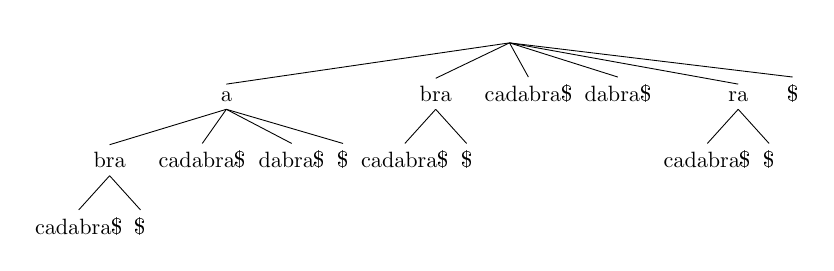
\begin{tikzpicture}[sibling distance=-1pt,scale=.8]
\Tree [.{}
[.a
    [.bra
        [.cadabra\$ ]
        [.\$ ]
    ]
    [.cadabra\$ ]
    [.dabra\$ ]
    [.\$ ]
]
[.bra
    [.cadabra\$ ]
    [.\$ ]
]
[.cadabra\$ ]
[.dabra\$ ]
[.ra
    [.cadabra\$ ]
    [.\$ ]
]
[.\$ ]
]
\end{tikzpicture}
\end{figure}
    
\end{frame}

\begin{frame}[fragile]
\frametitle{Autômato de Sufixos}

Autômato que aceita todos os sufixos de uma string.

\begin{figure}
\centering
\scalebox{.75}{
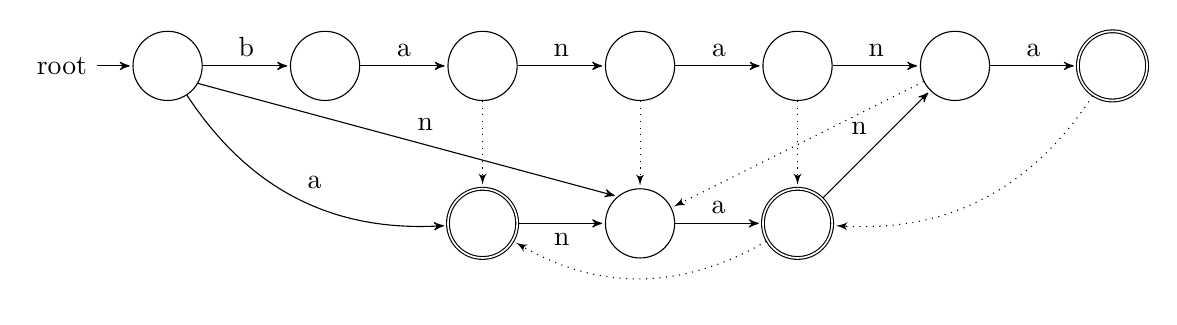
\begin{tikzpicture}[->,>=stealth',shorten >=1pt,node distance=2cm, auto, initial text={root}]
\node[initial, state] (0) {};
\node[state] (1) [right of=0] {};
\node[state] (2) [right of=1] {};
\node[state] (3) [right of=2] {};
\node[state] (4) [right of=3] {};
\node[state] (5) [right of=4] {};
\node[state,accepting] (6) [right of=5] {};
\node[state,accepting] (7) [below of=2] {};
\node[state] (8) [below of=3] {};
\node[state,accepting] (9) [below of=4] {};


\path (0) edge              node {b} (1)
      (0) edge [bend right] node {a} (7)
      (0.-30) edge          node {n} (8.130)
      (1) edge              node {a} (2)
      (2) edge              node {n} (3)
      (3) edge              node {a} (4)
      (4) edge              node {n} (5)
      (5) edge              node {a} (6)
      (7) edge              node[below] {n} (8)
      (8) edge              node {a} (9)
      (9) edge              node {n} (5);

\path (2) edge [dotted,>=latex']             node {} (7)
      (3) edge [dotted,>=latex']             node {} (8)
      (4) edge [dotted,>=latex']             node {} (9)
      (5) edge [dotted,>=latex']             node {} (8)
      (6) edge [dotted,>=latex',bend left]   node {} (9)
      (9) edge [dotted,>=latex',bend left]   node {} (7);

\end{tikzpicture}}
\end{figure}

\end{frame}

%\section{Árvore de sufixos}
%
%\begin{frame}[fragile]
%\frametitle{Introdução}
%
%\alert{Problema:} Dada~$S$, queremos saber se~$S$ ocorre na string~$T$, onde~$T$ é uma string conhecida.
%
%\pause
%Algoritmos conhecidos como KMP resolvem esse problema em tempo~$\Oh(|T| + |S|)$.
%
%Porém, se temos uma trie com todos os sufixos de~$T$, então~$S$ ocorre em~$T$ se e somente se existe um caminho nessa trie seguindo pelos caracteres de~$S$. Isso pode ser verificado em tempo~$\Oh(|S|)$, independente de~$|T|$.
%
%\end{frame}
%
%\begin{frame}[fragile]
%\frametitle{Estrutura}
%
%Essa trie, porém, consome espaço~$\Oh(|T|^2)$.
%
%Comprimindo os nós com grau de saída~$1$, cada nó restante tem grau de saída pelo menos 2, e assim a árvore tem no máximo~$2|T|$ nós.
%
%\begin{center}
%\begin{tikzpicture}
%\Tree [.{}
%[.a [.na [.nax ] [.x ] ] [.x ] ]
%[.bananax ]
%[.na [.nax ] [.x ] ]
%[.x ]
%]
%\end{tikzpicture}
%\end{center}
%
%Usando uma ordem inteligente de adicionar os sufixos, de forma a economizar operações, é possível construir esta árvore de sufixos com consumo de tempo~$\Oh(|S||\E|)$.
%
%\end{frame}

\plain{}{\alert{Perguntas?}}

\end{document}
